% arara: pdflatex: { shell: yes }
% arara: bibtex
% arara: pdflatex
% arara: pdflatex: { synctex: on}
% arara: clean: {files: [.aux, .idx, .ilg, .ind, .log, .bbl, .bcf, .ist, .blg, .run.xml]}

% sample.tex
% 
% A sample UMBCposter.
%
% Rouben Rostamian, February 2010

\documentclass[paper=a0paper, dvipsnames, fontmag=0.65]{umbcposter}
\usepackage{color}
\usepackage{enumitem}
\usepackage{colortbl}
\usepackage{tipa}
\usepackage{times}
\usepackage{graphicx}
\usepackage{url}
\usepackage{mdwlist}
\usepackage{amsmath,amsthm,amssymb,bm}
\usepackage{tikz}
\usetikzlibrary{spy,arrows.meta,shapes.geometric,arrows,fit ,plotmarks ,shapes.arrows,decorations.pathmorphing ,matrix,chains,scopes,positioning ,fadings ,patterns ,shapes,snakes,decorations.pathreplacing}
\tikzfading[name=fade out, inner color=transparent!0, outer color=transparent!100]

\usepackage[latin1]{inputenc}

\renewcommand{\rmdefault}{pag}

% Turn off indenting
\setlength{\parindent}{0in}

\let\Textsize\tiny
\def\Head#1{\noindent{\Large #1}}
\def\LHead#1{\noindent{\Large  #1}}
\def\Subhead#1{\noindent{\large #1}}
\def\Title#1{\noindent{\VeryHuge #1}}

\newcommand{\Line}{\hrulefill\par}
\newcommand{\Space}{\vspace{0.1cm}}

\newcommand{\myvec}[1]{\pmb{#1}}
\newcommand{\mleEst}{\hat{\Theta}_{\textrm{MLE}}}
\newcommand{\est}{\hat{\Theta}}
\newcommand{\fn}[2]{#1 \left( #2 \right)}
\newcommand{\samplespace}{\mathbb{S}}
\newcommand{\argmax}{\arg\max}
\newcommand{\definedas}{:=}


\begin{document}

\newcommand{\mytitle}{
\begin{minipage}[t]{0.5\linewidth}
		\huge Comparing John Walker's 18th century grammatical categories against those of today with Treetagger 
\end{minipage}
\hspace{0.1cm}
\begin{minipage}[t]{0.4\linewidth}
	\large Francois HUANG\\
	\large Blanche MIRET\\
	\large Preethi SRINIVASAN\\
	\large Dao THAUVIN\\
	\large Univ Paris Diderot \--- Sorbonne Paris Cit\'{e}\\ 
\end{minipage}
}

\posterinit{
	%grid,
	columns = {2},
	title align = {left},
	background style = {left color = white!90!gray, right color = white},
	title = \mytitle,
	left logo = {},
	right logo = {
\includegraphics[height=0.55\headheight]{Logo_Universite.png}},
	box/border style = {draw = black},
    box/header font = {\Large\bf},
	box/header font color = {black},
	box/header style = {top color = white!50!gray,
	bottom color = white!50!gray, line width=1pt},
	box/body style = {bottom color = white!80!gray, top color = white!90!gray},
	box/all rounded,
}

\boxit{col = 0, at top, name = introduction}{Introduction}{
  As it is very well known, Treetagger (\textit{Helmut Schmid}, 1996) is a tool that is widely used in the Natural Language Processing domain to annotate multilingual corpora with POS taggers and lemma information. The purpose of this study is to find out whether Treetagger could learn the grammatical categories of John Walker's \textit{Critical Pronouncing Dictionary }(1791), and how it will react by tagging 20th century's corpora. 
}
\boxit{col = 0, below of=introduction, name = corpus}{Data}{
  The data used for this investigation are the Walker's Dictionary, used to produce a lexicon and a list of tags, a part of the Brown Corpus used to train treetagger and test . 
}

\boxit{col = 0,span=1, below of = corpus, name = workflow}{First Steps}{
  Brown Corpus's tagset and grammatical categories of Walker's dictionary don't match
because many categories changed or simply disappeared over the course of time.
In other words, Brown Corpus's tags of 20th century and Walker's tags of 18th century
are not always the same, it could possibly influence the result's accuracy. 
Some Walker's dictionary's words were not tagged. 37895 words were tagged and 879 were not. We deleted the untagged words from our lexicon. 



\begin{center}
\begin{tabular}{c|c|c}
\hline
 \rowcolor[gray]{.75}
\textbf{Token} & \textbf{Walker's grammatical categories} &  \textbf{Treetagger's POS tags} \\
\hline
Abacus & s. & NN \\
\hline
Beneficed & a. & VBN \\
\hline
To Fight & v. a. & VB \\
\hline
Foreworn & part. & JJ \\
\hline
To can  & v.a. & VB \\
\hline
\end{tabular}
\end{center}

}
\boxit{col = 0,span=1, below of = workflow, name = remarks}{Remarks on Walker's Dictionary}{
  \begin{center}
Over 38 000 words, these are the most used POS by Walker.
\vspace{2mm}

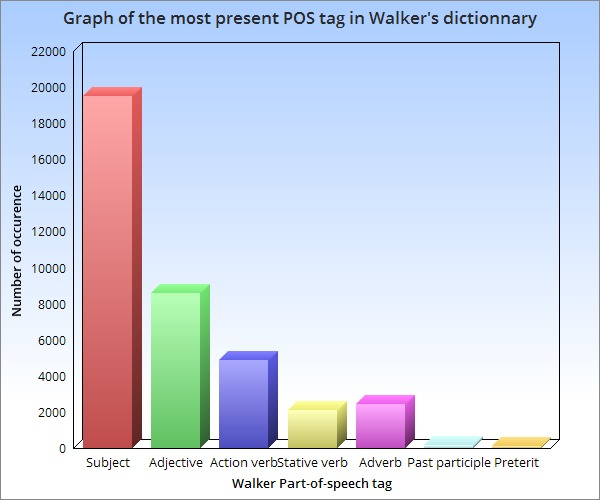
\includegraphics[width=8cm]{tagsetChart.jpeg}\\

\vspace{2mm}

Walker used many tags as Part-Of-Speech tags but the Brown Corpus doesn't consider all of them:
for e.g. there are no  \textit{plural, contraction} or \textit{A negative or privative termination.}\\

\vspace{2mm}

The word \textit{MEN} is tagged as \textbf{plural} but the word \textit{WOMEN} isn't.\\

\vspace{2mm}

The tag \textbf{contraction}  hasn't been used for every words which required it. For instance, the word \textit{NE'ER} is a poetical contraction for Never  and the word \textit{TA'EN} is a poetical contraction for Taken. While \textit{NE'ER} is declared as an adverb, \textit{TA'EN} is declared as a contraction.

\end{center}

}
\boxit{col = 0,span=1, below of = remarks, name = experience}{Experiment}{
  We mapped the Walker's Dictionary's grammatical categories with Brown Corpus tagset, 
the Brown Corpus's tags not used in the mapping were replaced by other tags of the Brown Corpus.
We applied this mapping on a part of the Brown Corpus.
We trained treetagger with that part of the Brown Corpus.
We tagged another part of the Brown Corpus with the obtained tagger and compared tags given by Brown Corpus and our tagger.
}
\boxit{col = 1,span=1, at top, name = preparingTT}{Preparing TreeTagger}{
  \centerline{\textbf{ About our lexicon :}}

	\vspace{0.5mm}
	
	We used the Walker's dictionary definitions to get the tagged words, we added some proper nouns, punctuation marks and cardinal numbers from our training set.
	
	\vspace{2mm}

\centerline{\textbf{Notes :}}

\begin{itemize}
	\item Walker's dictionary uses different tags for the same category.
	\item Some categories have disappeared, such as \textit{solemn nominative plural.} ( Hapax: Ye ), and \textit{A negative or privative termination.} ( Hapax: Less ).
\end{itemize}

		\vspace{2mm}

\centerline{\textbf{About our training set : }}
	\vspace{0.5mm}

	We borrowed a piece of the Brown corpus to train tree-tagger with about 1500 sentences and 28639 words (including punctuation marks).

\begin{center}
\begin{tabular}{c|c}
\hline
 \rowcolor[gray]{.75}
\textbf{Treetagger's POS tags} &  \textbf{Brown Corpus's POS tags} \\
\hline
art  &  at, dt \\
\hline
adj  &  jj, dti, ap, dts, jjt, jjr, jjs \\
\hline
pret  &  vbd, dod, bed, bedz, hvd \\
\hline
s  &  nn, nr, nns, nps \\
\hline
conj  &  in, cs, cc, dtx \\
\hline
prep  &  in, to \\
\hline
part.pass.  &  hvd, vbn, md \\
\hline
tp (third person)  &  vbz, bez, hvz, doz \\
\hline
v.  &  bem, vb, hv, be, do, ber \\
\hline
adv.  &   rb, ql, abx, abn, abl, ex \\
\hline
pron.  &  pps, ppo, pn, wps, ppl, wdt \\
\hline
part.  &  vbg \\
\hline
interj.  &  uh \\
\hline
\end{tabular}
\end{center}

}
\boxit{col = 1,span=1, below of = preparingTT, name = results}{Results}{
  We used our tree-tagger to tag a brown corpus text and compare with the tags given by the brown corpus.This is what we can observe :

\begin{description}

\item 1590 failures on 2332 tags.
\item A big amount of s. with 1300 failures in our tagging.
\item Only 8 tags have been used :
			adj., s., SENT, pron.pers., CD, NP, art., interj.

\end{description}

\begin{center}
	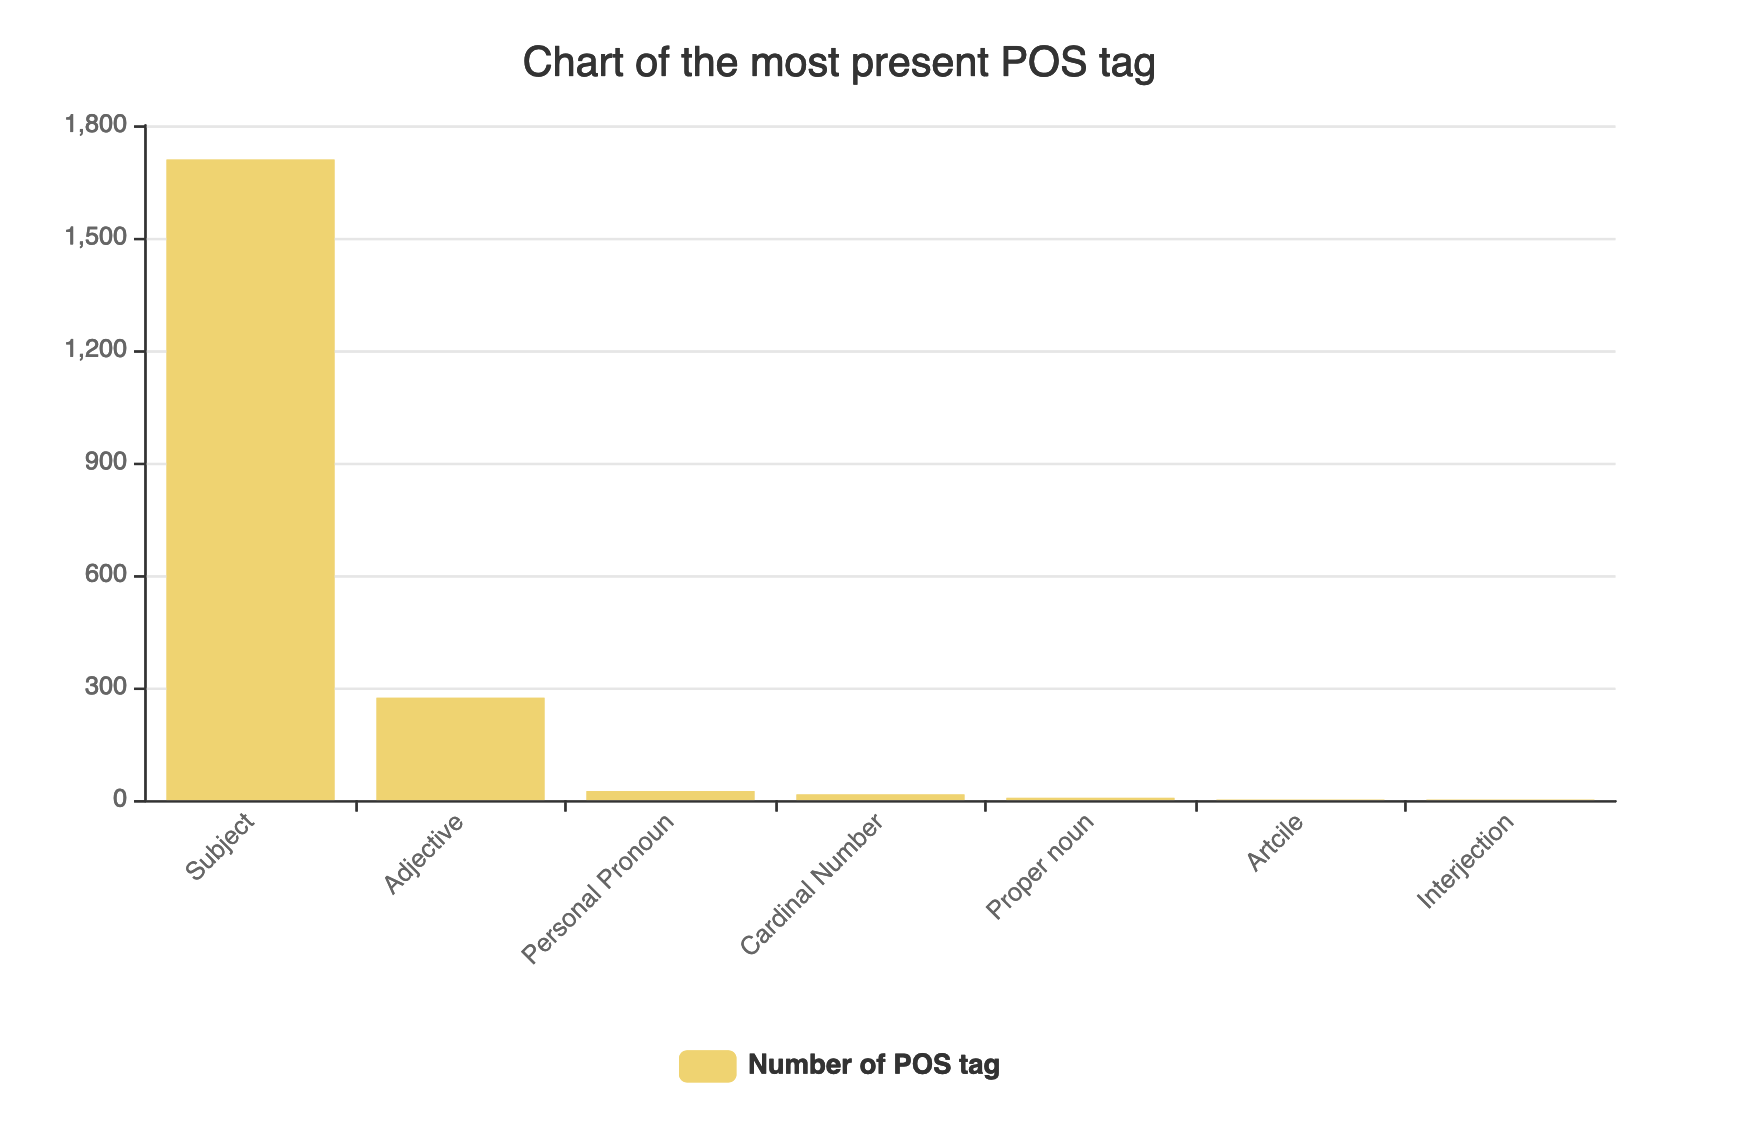
\includegraphics[width=8cm]{graphres.png}
\end{center}

}
\boxit{col = 1,span=1, below of = results, name = discuss}{Discussion about the results}{
  The tagset we obtained with our mapping has only 19 tags, compared to the Brown Corpus tagset size of 86 tags. Therefore, our small number of tags probably impacts the result.
Training on a bigger training set could give a better result. Most of the tags not used are rare tags that don't often appear in the training set. For example, the tag sp (for second person) appears only five times.\\
Our test set has only 2332 words (with punctuations), it is surely not enough to have an accurate result. In our case, even the number of failures is too  much for such a small amount of test data.
}
\boxit{col = 1,span=1, below of = discuss, name = references}{References}{
  \begin{enumerate}
\item J. Walker. \textit{A Critical Pronouncing Dictionary}, 1824.

\item N. Trapateau. \textit{A Critical Pronouncing Dictionary} from J. Walker xml file

\item W. N. Francis and H. Kucera. \textit{Brown Corpus}
\end{enumerate}
}



\end{document}

